\documentclass[11pt,a4paper]{article}

% ---------- packages ----------
\usepackage[utf8]{inputenc}
\usepackage[T1]{fontenc}
\usepackage{amsmath,amssymb}
\usepackage{graphicx}
\usepackage{booktabs}
\usepackage{hyperref}
\usepackage[margin=1in]{geometry}
\usepackage{caption}
\usepackage{subcaption}
\usepackage{listings}
\usepackage{xcolor}
\usepackage{float}
\usepackage{tikz}
\usetikzlibrary{shapes.geometric, arrows.meta, positioning, fit, backgrounds}

\lstset{
  basicstyle=\ttfamily\small,
  keywordstyle=\color{blue},
  commentstyle=\color{gray},
  breaklines=true,
  frame=single,
  numbers=left,
  numberstyle=\tiny\color{gray},
}

% ---------- title ----------
\title{Whip Dynamics: FEA Simulation and GNN Surrogate Modeling}
\author{LAU MeltFlow Project}
\date{\today}

\begin{document}
\maketitle

\begin{abstract}
This report documents the development of a finite-element-style simulation
of a bead chain (whip precursor) and the eventual training of a graph neural
network (GNN) surrogate solver. We record the formulations attempted, what
worked, what failed, and the rationale behind each design decision.
\end{abstract}

\tableofcontents
\newpage

% ==========================================================================
\section{Introduction and Motivation}
% ==========================================================================

The goal of this project is to:
\begin{enumerate}
    \item Build a physically accurate FEA-style simulation of a flexible
          chain/whip system.
    \item Use the simulation to generate graph-structured training data.
    \item Train a GNN to act as a surrogate solver, learning the
          physics from data rather than from explicit equations.
\end{enumerate}

The starting problem is a \textbf{bead chain released under gravity}: a
chain of $N$ mass nodes connected by rod elements, fixed to the ceiling at
one end, stretched horizontally, and released. This is a classical benchmark
that produces rich nonlinear dynamics (large rotations, wave propagation,
pendulum-like swinging) while remaining simple enough to validate.

% ==========================================================================
\section{Problem Setup}
% ==========================================================================

\subsection{Geometry and Initial Conditions}

\begin{itemize}
    \item $N = 16$ mass nodes connected by $N-1 = 15$ rod elements.
          (Power of 2 to support binary-tree GNN architecture.)
    \item Total chain length $L = 2.0\;\text{m}$, rest length per element
          $\ell_0 = L/(N-1)$.
    \item Total mass $M = 0.5\;\text{kg}$, distributed with a linear taper.
          Taper ratio $r = m_0 / m_{N-1}$ controls the mass gradient from
          base to tip ($r = 1$ for uniform, $r = 10$ for whip-like taper).
    \item Node 0 is fixed at the origin (ceiling anchor).
    \item Nodes $1 \ldots N-1$ are initially placed horizontally:
          $\mathbf{x}_i(0) = (i \cdot \ell_0,\; 0)$.
    \item Zero initial velocity: $\mathbf{v}_i(0) = \mathbf{0}$.
    \item Released under gravity $g = 9.81\;\text{m/s}^2$ acting in $-y$.
    \item Global velocity drag $\mathbf{F}_{\text{drag}} = -\beta\,\mathbf{v}$
          with $\beta = 0.02$ provides gentle settling.
\end{itemize}

\subsection{Graph Structure}

The finite element mesh is inherently a graph:
\begin{itemize}
    \item \textbf{Nodes}: mass points with features
          $(\mathbf{x}, \mathbf{v}, \text{node\_type})$.
    \item \textbf{Edges}: rod elements with features
          $(\ell_0, \text{current stretch})$.
    \item Edges stored bidirectionally for GNN message passing:
          $(i \to j)$ and $(j \to i)$ for each element.
\end{itemize}

This maps directly to a \texttt{torch\_geometric.data.Data} object for GNN
training.

% ==========================================================================
\section{Formulation Attempts}
\label{sec:formulations}
% ==========================================================================

We explored two fundamentally different approaches to enforcing the
near-inextensibility of the rod elements. This section documents both,
including what failed and why.

% ---------- 3.1 ----------
\subsection{Attempt 1: Position Verlet with SHAKE Constraints}
\label{sec:shake}

\subsubsection{Formulation}

The first approach treated the rods as \emph{rigid constraints} (exact
inextensibility) using the SHAKE algorithm paired with position-form
St\"ormer-Verlet integration:

\begin{align}
    \mathbf{x}_{n+1} &= 2\mathbf{x}_n - \mathbf{x}_{n-1}
                        + \Delta t^2 \, \mathbf{a}_n
    \label{eq:verlet_pos} \\
    \text{SHAKE:}\quad
    |\mathbf{x}_{n+1,j} - \mathbf{x}_{n+1,i}| &= \ell_0
    \quad \forall\; \text{element } (i,j)
    \label{eq:shake}
\end{align}

SHAKE iteratively projects positions onto the constraint manifold using
Gauss-Seidel sweeps along the chain:
\begin{align}
    \boldsymbol{\delta} &= \mathbf{x}_j - \mathbf{x}_i, \quad
    d = |\boldsymbol{\delta}| \\
    \text{correction} &= \frac{d - \ell_0}{d} \, \boldsymbol{\delta} \\
    \mathbf{x}_i &\mathrel{+}= \frac{w_i}{w_i + w_j} \, \text{correction}, \quad
    \mathbf{x}_j \mathrel{-}= \frac{w_j}{w_i + w_j} \, \text{correction}
\end{align}
where $w_i = 1/m_i$ is the inverse mass ($w_0 = 0$ for the fixed anchor).

\subsubsection{Results}

\begin{itemize}
    \item \textbf{Constraint satisfaction}: Good.
          Maximum relative length error $\sim 3 \times 10^{-5}$ with 20
          Gauss-Seidel iterations per timestep.
    \item \textbf{Energy conservation}: \textbf{Poor.}
          Total energy drifted by $\sim 1\;\text{J}$ over $5\;\text{s}$,
          even with $\Delta t = 0.0005\;\text{s}$ and 100 constraint
          iterations.
\end{itemize}

\subsubsection{Why It Failed}

The energy drift stemmed from the interaction between SHAKE and the velocity
update. Two specific issues:

\begin{enumerate}
    \item \textbf{Velocity Verlet variant}: Our initial implementation used
          velocity Verlet with SHAKE, but the standard SHAKE algorithm only
          corrects positions---it does not include the RATTLE velocity
          projection step needed to keep velocities tangent to the
          constraint manifold. Without RATTLE, the velocity gains a
          component along the constraint gradient each timestep, injecting
          energy.
    \item \textbf{Position Verlet variant}: Switching to pure position
          Verlet (Eq.~\ref{eq:verlet_pos}) avoids explicit velocities, but
          the Gauss-Seidel SHAKE projection converges slowly for chains:
          information propagates only one link per iteration. With 19
          links, even 100 iterations leave residual constraint errors that
          accumulate over thousands of timesteps.
\end{enumerate}

\subsubsection{Lessons Learned}

\begin{itemize}
    \item SHAKE/RATTLE is well-suited to molecular dynamics where bonds are
          short and constraint graphs are sparse, but performs poorly on
          long serial chains.
    \item For a chain of $N$ nodes, convergence requires $O(N)$ iterations
          per step, making it inefficient.
    \item The lack of a tunable stiffness parameter is elegant but makes
          debugging and validation harder.
\end{itemize}

% ---------- 3.2 ----------
\subsection{Attempt 2: Symplectic Euler with Penalty Springs}
\label{sec:symplectic}

\subsubsection{Formulation}

The second (and successful) approach replaces rigid constraints with stiff
Hookean springs. Each rod element exerts a force:

\begin{equation}
    \mathbf{F}_{ij}^{\text{spring}} = k \, (d - \ell_0) \, \hat{\boldsymbol{\delta}}
    \label{eq:spring}
\end{equation}

where $k$ is the spring stiffness, $d = |\mathbf{x}_j - \mathbf{x}_i|$,
and $\hat{\boldsymbol{\delta}} = (\mathbf{x}_j - \mathbf{x}_i)/d$.

Optional viscous damping along the rod axis:

\begin{equation}
    \mathbf{F}_{ij}^{\text{damp}} = c \,
    \bigl((\mathbf{v}_j - \mathbf{v}_i) \cdot \hat{\boldsymbol{\delta}}\bigr)
    \, \hat{\boldsymbol{\delta}}
    \label{eq:damping}
\end{equation}

Time integration uses symplectic (semi-implicit) Euler:

\begin{align}
    \mathbf{v}_{n+1} &= \mathbf{v}_n + \Delta t \, \mathbf{a}(\mathbf{x}_n)
    \label{eq:symp_v} \\
    \mathbf{x}_{n+1} &= \mathbf{x}_n + \Delta t \, \mathbf{v}_{n+1}
    \label{eq:symp_x}
\end{align}

Note the key difference from explicit Euler: the position update uses the
\emph{new} velocity $\mathbf{v}_{n+1}$, not $\mathbf{v}_n$. This makes the
scheme symplectic.

\subsubsection{Walkthrough: Updating a Single Bead}

To build intuition, we trace exactly what happens to one interior bead $i$
(not the fixed anchor) during a single timestep. At the start of the step,
bead $i$ has position $\mathbf{x}_i$, velocity $\mathbf{v}_i$, and mass $m$.

\paragraph{Step 1: Compute all forces on bead $i$.}
Three types of force act on it:

\begin{enumerate}
    \item \textbf{Gravity}, pulling it downward:
    \begin{equation}
        \mathbf{F}^{\text{grav}}_i = \bigl(0,\; -mg\bigr)
    \end{equation}

    \item \textbf{Spring from the left neighbor} (bead $i-1$).
    The rod connecting them has rest length $\ell_0$. If the current
    distance $d = |\mathbf{x}_i - \mathbf{x}_{i-1}|$ differs from
    $\ell_0$, the spring pulls them back together (or pushes them apart):
    \begin{equation}
        \mathbf{F}^{\text{left}}_i
        = -k\,(d - \ell_0)\,\hat{\boldsymbol{\delta}}
    \end{equation}
    where $\hat{\boldsymbol{\delta}}$ points from bead $i{-}1$ to bead $i$.
    When the rod is stretched ($d > \ell_0$), this force pulls bead $i$
    back toward its neighbor.

    \item \textbf{Spring from the right neighbor} (bead $i+1$). Same
    formula, opposite direction.
\end{enumerate}

An optional viscous \textbf{damping} force along each rod resists relative
motion between neighbors. The total force is:
\begin{equation}
    \mathbf{F}_i = \mathbf{F}^{\text{grav}}_i
                 + \mathbf{F}^{\text{left}}_i
                 + \mathbf{F}^{\text{right}}_i
                 + \mathbf{F}^{\text{damp}}_i
\end{equation}

\paragraph{Step 2: Acceleration} from Newton's second law:
\begin{equation}
    \mathbf{a}_i = \frac{\mathbf{F}_i}{m}
\end{equation}

\paragraph{Step 3: Update velocity \emph{first}.}
\begin{equation}
    \mathbf{v}_i^{\text{new}}
    = \mathbf{v}_i + \Delta t \;\mathbf{a}_i
\end{equation}

\paragraph{Step 4: Update position using the \emph{new} velocity.}
\begin{equation}
    \mathbf{x}_i^{\text{new}}
    = \mathbf{x}_i + \Delta t \;\mathbf{v}_i^{\text{new}}
\end{equation}

The ordering---velocity first, then position with the updated velocity---is
what makes this \emph{symplectic} Euler rather than plain (explicit) Euler.
A small difference in code, but it is what keeps the total energy from
drifting over long simulations.

\paragraph{Numerical example.}
Suppose bead~5 is at $\mathbf{x} = (0.5,\, -0.3)$ with velocity
$\mathbf{v} = (0.1,\, -2.0)\;\text{m/s}$, and the total force on it works
out to $\mathbf{F} = (3.0,\, -4.0)\;\text{N}$ with
$m = 0.025\;\text{kg}$:

\begin{align}
    \mathbf{a}
      &= \frac{(3.0,\;-4.0)}{0.025}
       = (120,\;-160)\;\text{m/s}^2 \\[6pt]
    \mathbf{v}^{\text{new}}
      &= (0.1,\;-2.0) + 0.0001 \times (120,\;-160)
       = (0.112,\;-2.016)\;\text{m/s} \\[6pt]
    \mathbf{x}^{\text{new}}
      &= (0.5,\;-0.3) + 0.0001 \times (0.112,\;-2.016)
       = (0.500011,\;-0.300202)\;\text{m}
\end{align}

Each bead moves a tiny amount per step. With $\Delta t = 0.0001\;\text{s}$
and a $5\;\text{s}$ simulation, we take 50{,}000 such steps. Each step is
the same simple sequence: forces $\to$ acceleration $\to$ new velocity
$\to$ new position.

\subsubsection{Parameters}

\begin{table}[H]
\centering
\begin{tabular}{lrl}
\toprule
Parameter & Value & Notes \\
\midrule
Stiffness $k$ & $10{,}000\;\text{N/m}$ & High enough for $<1\%$ stretch \\
Damping $c$ & $0.5$ & Physical energy dissipation \\
Timestep $\Delta t$ & $0.0001\;\text{s}$ & Stable for $k=10^4$ \\
Duration & $5.0\;\text{s}$ & ${\sim}1.75$ swing periods \\
Save interval & 50 steps & 1001 output frames \\
\bottomrule
\end{tabular}
\caption{Default simulation parameters.}
\label{tab:params}
\end{table}

\subsubsection{Stability Criterion}

For symplectic Euler with a spring of stiffness $k$ and mass $m$, the
stability limit is:

\begin{equation}
    \Delta t < 2\sqrt{\frac{m}{k}}
    = 2\sqrt{\frac{0.025}{10{,}000}}
    = 0.00316\;\text{s}
\end{equation}

Our timestep $\Delta t = 0.0001\;\text{s}$ is well within this limit
(factor of 31$\times$ safety margin).

\subsubsection{Results}

\begin{itemize}
    \item \textbf{Energy conservation (undamped, $c=0$)}: Excellent.
          Total energy oscillates within $\pm 0.04\;\text{J}$ over
          $5\;\text{s}$ with no systematic drift. This is the expected
          behavior for a symplectic integrator.
    \item \textbf{Energy dissipation (damped, $c=0.5$)}: Total energy
          decreases monotonically from $0$ to $\sim -1.6\;\text{J}$,
          confirming the damping acts as a physical energy sink.
    \item \textbf{Constraint satisfaction}: Maximum rod stretch $<1\%$ at
          $k = 10^4$. Occasional peaks to $\sim 3\%$ during high-velocity
          events (tip snap).
    \item \textbf{Qualitative behavior}: Chain falls, swings through the
          vertical, overshoots to the opposite side, and gradually settles
          due to damping. Physically correct.
\end{itemize}

\subsubsection{Why It Works}

\begin{enumerate}
    \item \textbf{Symplectic structure}: The semi-implicit Euler scheme
          preserves the symplectic form of Hamiltonian mechanics, meaning
          energy oscillates around the true value but doesn't drift.
    \item \textbf{No iterative projection}: Unlike SHAKE, there is no
          iterative constraint solve. Forces are computed explicitly from
          positions, making each timestep $O(N)$ with a small constant.
    \item \textbf{Tunable stiffness}: The spring constant $k$ provides a
          direct physical knob. Increasing $k$ reduces stretch at the cost
          of requiring smaller $\Delta t$.
    \item \textbf{GNN compatibility}: The force computation
          (Eq.~\ref{eq:spring}) is a local, pairwise message along edges
          --- exactly the computation a GNN learns to approximate.
\end{enumerate}

% ==========================================================================
\section{Implementation}
% ==========================================================================

\subsection{Code Structure}

\begin{table}[H]
\centering
\begin{tabular}{ll}
\toprule
File & Purpose \\
\midrule
\texttt{simulation.py} & Chain state, force computation, time integration \\
\texttt{visualize.py}   & Matplotlib animation and energy diagnostics \\
\texttt{main.py}        & CLI runner, parameter config, \texttt{.npz} export \\
\bottomrule
\end{tabular}
\caption{Source files.}
\end{table}

\subsection{Data Export Format}

Simulation output is saved as a NumPy \texttt{.npz} archive with the
following arrays, designed for direct consumption by a GNN:

\begin{table}[H]
\centering
\begin{tabular}{lll}
\toprule
Key & Shape & Description \\
\midrule
\texttt{positions}      & $(T, N, 2)$ & Node positions per frame \\
\texttt{velocities}     & $(T, N, 2)$ & Node velocities per frame \\
\texttt{accelerations}  & $(T, N, 2)$ & Node accelerations (training target) \\
\texttt{edge\_index}    & $(2, 2E)$   & Bidirectional edge connectivity \\
\texttt{node\_types}    & $(N,)$      & $0$ = free, $1$ = fixed \\
\texttt{rest\_lengths}  & $(E,)$      & Element rest lengths \\
\texttt{times}          & $(T,)$      & Timestamps \\
\bottomrule
\end{tabular}
\caption{Data export format. $T$ = saved frames, $N$ = nodes, $E$ = elements.}
\label{tab:data}
\end{table}

Scalar metadata (\texttt{dt}, \texttt{gravity}, \texttt{stiffness},
\texttt{damping}, \texttt{n\_nodes}, etc.) is also included.

% ==========================================================================
\section{Qt/C++ Implementation: Signal/Slot Message Passing}
\label{sec:qt}
% ==========================================================================

The Qt implementation mirrors the Python physics exactly but structures the
computation as \emph{local per-node operations} coordinated by a central
simulator---directly analogous to a GNN's message-passing architecture. This
section documents which operations occur inside each bead (node-local) versus
which require global coordination.

\subsection{Architecture Overview}

The simulation consists of three object types:

\begin{itemize}
    \item \textbf{\texttt{Bead}} --- a \texttt{QObject} representing a single
          mass node. Each bead owns its position $\mathbf{x}$, velocity
          $\mathbf{v}$, mass $m$, and a force accumulator
          $\mathbf{F}_{\text{accum}}$. Beads communicate via Qt signals and
          slots.
    \item \textbf{\texttt{Rod}} --- a lightweight struct storing edge
          connectivity (two bead indices) and rest length $\ell_0$. Rods have
          no behavior; they define the graph topology.
    \item \textbf{\texttt{ChainSimulator}} --- the coordinator that owns all
          beads and rods, drives the timestep, and manages global operations.
\end{itemize}

\subsection{Per-Bead Operations (Node-Local)}

Each bead performs the following operations using \emph{only its own state}
and \emph{messages received from immediate neighbors}. These are implemented
as Qt slots on the \texttt{Bead} class:

\subsubsection{\texttt{resetForces()}}
Zeros the force accumulator: $\mathbf{F}_{\text{accum}} \leftarrow \mathbf{0}$.

\subsubsection{\texttt{applyGravity(g)}}
Adds gravitational force using only the bead's own mass:
\begin{equation}
    \mathbf{F}_{\text{accum}} \mathrel{+}= (0,\; -mg)
\end{equation}
If a global drag coefficient $\beta > 0$ is set, also applies velocity drag:
\begin{equation}
    \mathbf{F}_{\text{accum}} \mathrel{-}= \beta \, \mathbf{v}
\end{equation}
Fixed beads skip this entirely.

\subsubsection{\texttt{onNeighborState(neighborPos, neighborVel, $\ell_0$)}}
\label{sec:message}

This is the \textbf{message-passing function}---the GNN analogue of an edge
message followed by aggregation. When a bead receives a neighbor's state, it
computes the spring and damping forces from that single neighbor and adds them
to its accumulator:

\begin{align}
    \boldsymbol{\delta} &= \mathbf{x}_{\text{neighbor}} - \mathbf{x}_{\text{self}} \\
    d &= |\boldsymbol{\delta}|, \quad \hat{\mathbf{d}} = \boldsymbol{\delta}/d \\
    \mathbf{F}_{\text{accum}} &\mathrel{+}= k\,(d - \ell_0)\,\hat{\mathbf{d}}
        \quad\text{(spring)} \\
    \mathbf{F}_{\text{accum}} &\mathrel{+}= c\,\bigl((\mathbf{v}_{\text{neighbor}}
        - \mathbf{v}_{\text{self}}) \cdot \hat{\mathbf{d}}\bigr)\,\hat{\mathbf{d}}
        \quad\text{(damping)}
\end{align}

This slot is called once per neighbor per timestep. For an interior bead with
two neighbors, the accumulator sums two spring/damping contributions. The
bead does \emph{not} know how many neighbors it has or where they are in the
chain---it simply accumulates whatever messages arrive.

\subsubsection{\texttt{integrate(dt)}}
The \textbf{node update function}. Using only its own accumulated force and
mass, the bead updates its state via symplectic Euler:
\begin{align}
    \mathbf{a} &= \mathbf{F}_{\text{accum}} / m \\
    \mathbf{v} &\mathrel{+}= \Delta t \, \mathbf{a} \\
    \mathbf{x} &\mathrel{+}= \Delta t \, \mathbf{v}
\end{align}
Fixed beads zero their force accumulator and return without moving.

\subsection{Global Operations (Simulator-Level)}

The \texttt{ChainSimulator} performs three operations that require knowledge
of the full graph structure. These cannot be decomposed into independent
per-node computations.

\subsubsection{Phase 1: Message Dispatch}

The simulator iterates over all rods (edges) and calls
\texttt{onNeighborState} on both endpoints:

\begin{lstlisting}[language=C++,caption={Message dispatch in ChainSimulator::step()}]
for (const Rod &rod : m_rods) {
    Bead *a = m_beads[rod.beadA];
    Bead *b = m_beads[rod.beadB];
    b->onNeighborState(a->id(), a->pos(), a->vel(), rod.restLength);
    a->onNeighborState(b->id(), b->pos(), b->vel(), rod.restLength);
}
\end{lstlisting}

This is the coordinator role: the simulator knows the graph topology (which
beads are connected) and orchestrates message delivery. The beads themselves
are topology-unaware.

\subsubsection{Phase 2: Synchronized Integration}

After all messages have been delivered and forces accumulated, the simulator
triggers integration on all beads simultaneously:

\begin{lstlisting}[language=C++]
for (Bead *b : m_beads)
    b->integrate(dt);
\end{lstlisting}

The synchronization matters: all beads must finish accumulating forces before
any bead updates its position. This prevents order-dependent results and
mirrors the synchronous update in a GNN forward pass.

\subsubsection{Phase 3: Constraint Projection (SHAKE)}
\label{sec:qt_shake}

After integration, the simulator optionally runs an iterative SHAKE projection
over all rods to enforce inextensibility. This is fundamentally
\textbf{non-local}: correcting one rod's length changes the positions of its
endpoints, which affects adjacent rods. The algorithm iterates until
convergence:

\begin{lstlisting}[language=C++,caption={SHAKE constraint projection (simplified)}]
for (int iter = 0; iter < maxIters; ++iter) {
    for (const Rod &rod : m_rods) {
        // read both endpoints, compute length error,
        // adjust both positions proportional to inverse mass
    }
    if (maxError < tolerance) break;
}
// then correct velocities along each rod
\end{lstlisting}

This phase has no direct analogue in a single-layer GNN. It requires:
\begin{itemize}
    \item Reading and writing \emph{pairs} of nodes simultaneously
    \item Multiple iterations over the entire edge set
    \item Convergence-dependent termination
\end{itemize}

A flat GNN would need $O(N)$ message-passing layers to approximate what SHAKE
achieves in ${\sim}10$ iterations. This motivates the hierarchical
binary-tree architecture described in Section~\ref{sec:tree_gnn}.

\subsection{Summary: Local vs.\ Global}

\begin{table}[H]
\centering
\begin{tabular}{lll}
\toprule
Operation & Scope & GNN Analogue \\
\midrule
\texttt{resetForces()} & Node-local & Reset hidden state \\
\texttt{applyGravity(g)} & Node-local & Node feature (external force) \\
\texttt{onNeighborState()} & Node-local (1-hop) & Edge message + aggregation \\
\texttt{integrate(dt)} & Node-local & Node update function \\
\midrule
Message dispatch & Global (topology) & GNN layer coordination \\
Synchronized integration & Global (ordering) & Synchronous update \\
SHAKE projection & Global (iterative) & \textbf{No single-layer analogue} \\
\bottomrule
\end{tabular}
\caption{Classification of simulation operations by scope.}
\label{tab:local_global}
\end{table}

The first four operations---everything inside the \texttt{Bead} class---map
directly to a standard GNN layer. The last three are coordinator
responsibilities. Of these, message dispatch and synchronization are handled
by any GNN framework automatically. Only the SHAKE constraint projection
requires architectural innovation (hierarchical message passing) to capture.

\subsection{Timestep Flowchart}

Figure~\ref{fig:flowchart} shows a single timestep as a threading diagram.
The left lane represents the \texttt{Bead} objects (child threads, running in
parallel), and the right lane represents the \texttt{ChainSimulator}
(parent/coordinator thread). Horizontal dashed lines are synchronization
barriers where the coordinator waits for all beads to finish before
proceeding. Diagonal arrows show data flow between the two lanes.

\begin{figure}[H]
\centering
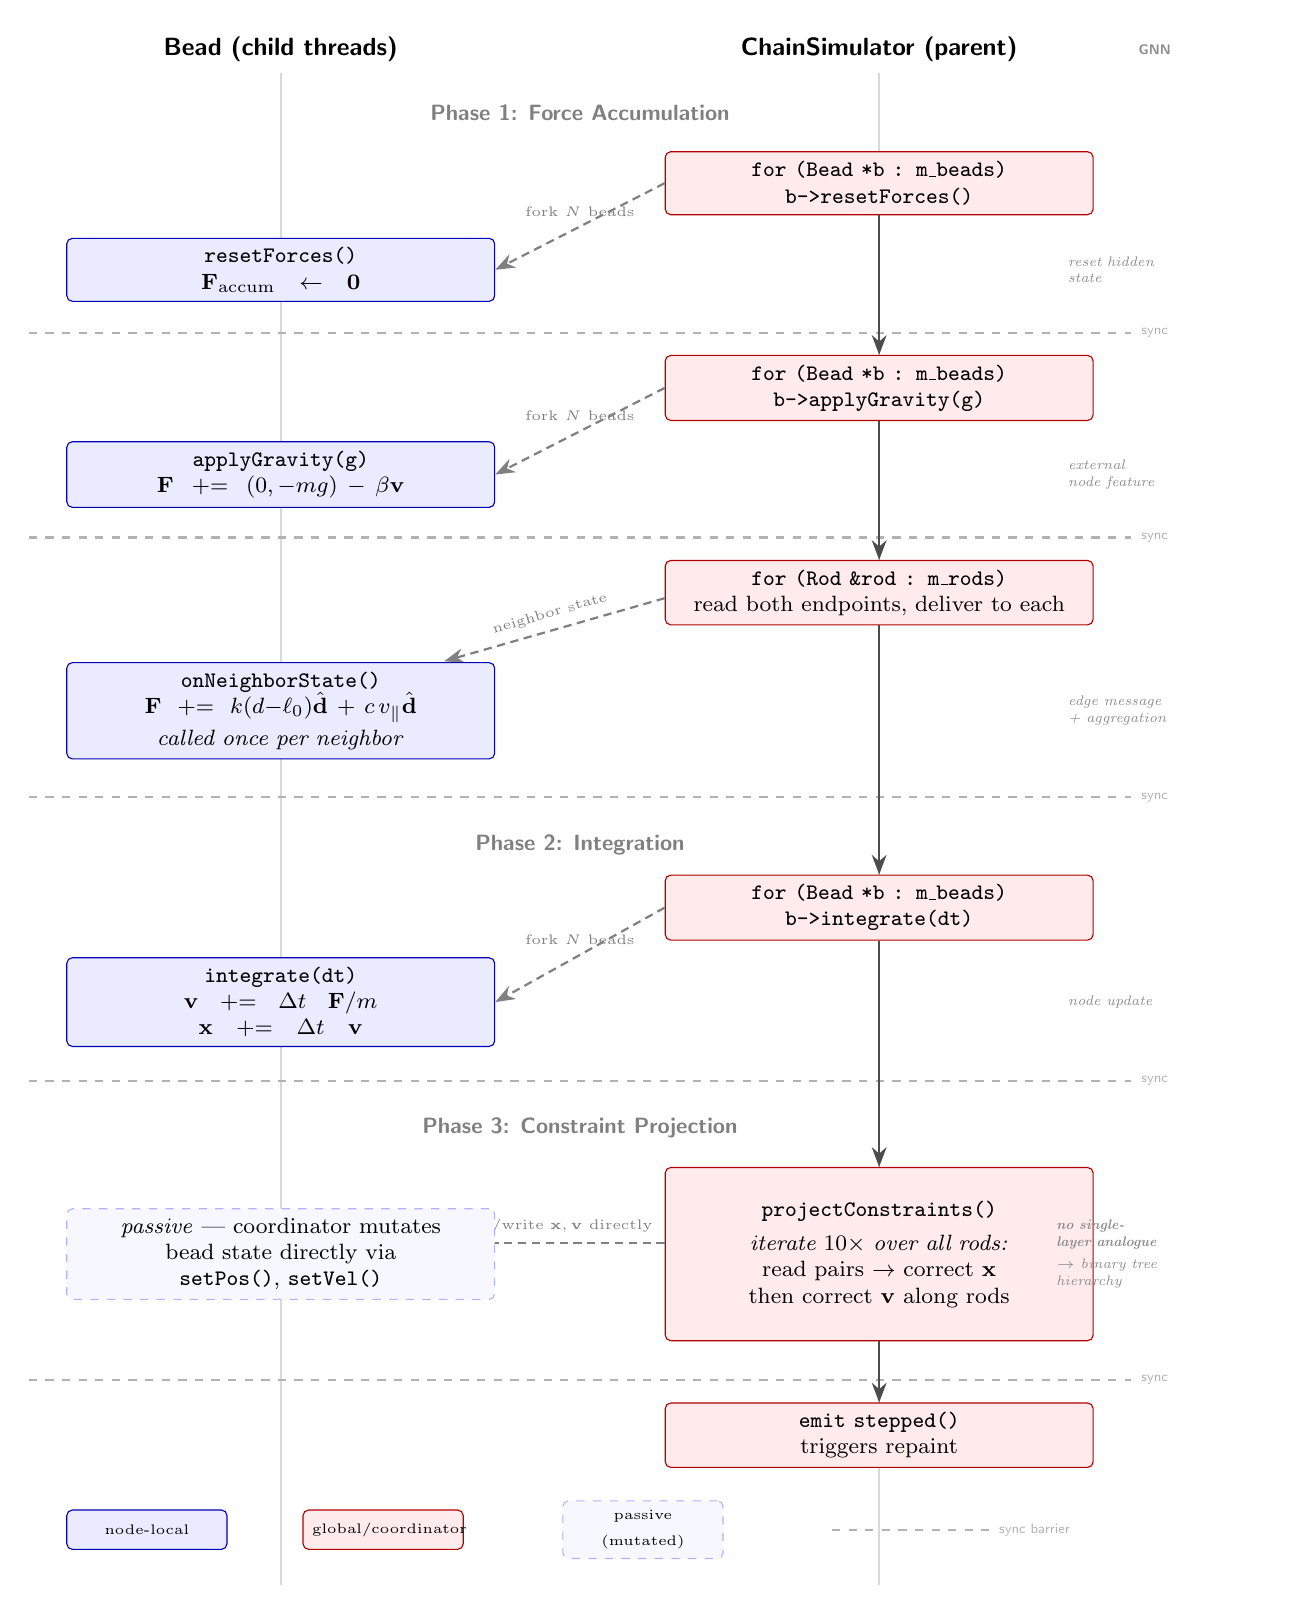
\begin{tikzpicture}[
    >={Stealth[length=2.5mm]},
    % Bead lane boxes (blue)
    bead/.style={
        rectangle, rounded corners=2pt, draw=blue!70!black, fill=blue!8,
        text width=5.2cm, minimum height=0.8cm, align=center,
        font=\footnotesize
    },
    % Coordinator lane boxes (red)
    coord/.style={
        rectangle, rounded corners=2pt, draw=red!70!black, fill=red!8,
        text width=5.2cm, minimum height=0.8cm, align=center,
        font=\footnotesize
    },
    % Sync barrier
    barrier/.style={
        dashed, gray!60, thick
    },
    % Cross-lane arrow
    xarr/.style={->, thick, black!50, densely dashed},
    % Vertical arrow
    varr/.style={->, thick, black!70},
    % Lane header
    header/.style={
        font=\small\bfseries\sffamily, fill=white
    },
    % Phase label
    phase/.style={
        font=\footnotesize\bfseries\sffamily, text=black!50
    },
    % GNN annotation
    gnn/.style={
        font=\tiny\itshape, text=black!45, text width=2.2cm, align=left
    },
]

% Column centers
\def\beadx{-3.8}
\def\coordx{3.8}
\def\gnnx{7.3}

% Lane headers
\node[header] at (\beadx, 0.3) {Bead (child threads)};
\node[header] at (\coordx, 0.3) {ChainSimulator (parent)};
\node[header, text=black!45] at (\gnnx, 0.3) {\tiny GNN};

% Lane lines
\draw[gray!30, thick] (\beadx, 0) -- (\beadx, -19.2);
\draw[gray!30, thick] (\coordx, 0) -- (\coordx, -19.2);

% ===== Phase 1: Force Accumulation =====
\node[phase] at (0, -0.5) {Phase 1: Force Accumulation};

% 1a: Coordinator triggers reset
\node[coord] (c_reset) at (\coordx, -1.4)
    {\texttt{for (Bead *b : m\_beads)} \\ \texttt{b->resetForces()}};

\node[bead] (b_reset) at (\beadx, -2.5)
    {\texttt{resetForces()} \\ $\mathbf{F}_{\text{accum}} \leftarrow \mathbf{0}$};

\draw[xarr] (c_reset.west) -- (b_reset.east)
    node[midway, above, font=\tiny, text=black!50] {fork $N$ beads};

\node[gnn] at (\gnnx, -2.5) {reset hidden\\state};

% Barrier 1
\draw[barrier] (-7, -3.3) -- (7, -3.3)
    node[right, font=\tiny\sffamily, text=gray!60] {sync};

% 1b: Coordinator triggers gravity
\node[coord] (c_grav) at (\coordx, -4.0)
    {\texttt{for (Bead *b : m\_beads)} \\ \texttt{b->applyGravity(g)}};

\node[bead] (b_grav) at (\beadx, -5.1)
    {\texttt{applyGravity(g)} \\ $\mathbf{F} \mathrel{+}= (0, -mg) - \beta\mathbf{v}$};

\draw[xarr] (c_grav.west) -- (b_grav.east)
    node[midway, above, font=\tiny, text=black!50] {fork $N$ beads};

\node[gnn] at (\gnnx, -5.1) {external\\node feature};

% Barrier 2
\draw[barrier] (-7, -5.9) -- (7, -5.9)
    node[right, font=\tiny\sffamily, text=gray!60] {sync};

% 1c: Coordinator dispatches messages
\node[coord] (c_msg) at (\coordx, -6.6)
    {\texttt{for (Rod \&rod : m\_rods)} \\ read both endpoints, deliver to each};

\draw[xarr] ([yshift=-2pt]c_msg.west) -- +(-2.8, -0.8)
    node[midway, above, font=\tiny, text=black!50, sloped] {neighbor state};

\node[bead] (b_msg) at (\beadx, -8.1)
    {\texttt{onNeighborState()} \\
     $\mathbf{F} \mathrel{+}= k(d{-}\ell_0)\hat{\mathbf{d}} + c\,v_\parallel\hat{\mathbf{d}}$ \\[2pt]
     \textit{called once per neighbor}};

\node[gnn] at (\gnnx, -8.1) {edge message\\+ aggregation};

% Barrier 3
\draw[barrier] (-7, -9.2) -- (7, -9.2)
    node[right, font=\tiny\sffamily, text=gray!60] {sync};

% ===== Phase 2: Integration =====
\node[phase] at (0, -9.8) {Phase 2: Integration};

\node[coord] (c_int) at (\coordx, -10.6)
    {\texttt{for (Bead *b : m\_beads)} \\ \texttt{b->integrate(dt)}};

\node[bead] (b_int) at (\beadx, -11.8)
    {\texttt{integrate(dt)} \\
     $\mathbf{v} \mathrel{+}= \Delta t\;\mathbf{F}/m$ \\
     $\mathbf{x} \mathrel{+}= \Delta t\;\mathbf{v}$};

\draw[xarr] (c_int.west) -- (b_int.east)
    node[midway, above, font=\tiny, text=black!50] {fork $N$ beads};

\node[gnn] at (\gnnx, -11.8) {node update};

% Barrier 4
\draw[barrier] (-7, -12.8) -- (7, -12.8)
    node[right, font=\tiny\sffamily, text=gray!60] {sync};

% ===== Phase 3: Constraint Projection =====
\node[phase] at (0, -13.4) {Phase 3: Constraint Projection};

\node[coord, minimum height=2.2cm] (c_shake) at (\coordx, -15.0)
    {\texttt{projectConstraints()} \\[3pt]
     \textit{iterate $10\times$ over all rods:} \\
     read pairs $\to$ correct $\mathbf{x}$ \\
     then correct $\mathbf{v}$ along rods};

% Shake reads/writes beads directly
\draw[xarr] ([yshift=4pt]c_shake.west) -- +(-2.8, 0)
    node[midway, above, font=\tiny, text=black!50] {read/write $\mathbf{x},\mathbf{v}$ directly};

\node[bead, dashed, draw=blue!30, fill=blue!3] (b_passive) at (\beadx, -15.0)
    {\textit{passive} --- coordinator mutates \\ bead state directly via \\ \texttt{setPos()}, \texttt{setVel()}};

\node[gnn, text width=2.5cm] at (\gnnx, -15.0) {\textbf{no single-}\\
    \textbf{layer analogue}\\[2pt] $\to$ binary tree\\hierarchy};

% Barrier 5
\draw[barrier] (-7, -16.6) -- (7, -16.6)
    node[right, font=\tiny\sffamily, text=gray!60] {sync};

% ===== End =====
\node[coord] (c_end) at (\coordx, -17.3)
    {\texttt{emit stepped()} \\ triggers repaint};

% Vertical flow arrows (coordinator side)
\draw[varr] (c_reset) -- (c_grav);
\draw[varr] (c_grav) -- (c_msg);
\draw[varr] (c_msg) -- (c_int);
\draw[varr] (c_int) -- (c_shake);
\draw[varr] (c_shake) -- (c_end);

% Legend
\node[bead, text width=1.8cm, minimum height=0.5cm] at (-5.5, -18.5) {\tiny node-local};
\node[coord, text width=1.8cm, minimum height=0.5cm] at (-2.5, -18.5) {\tiny global/coordinator};
\node[bead, dashed, draw=blue!30, fill=blue!3, text width=1.8cm, minimum height=0.5cm]
    at (0.8, -18.5) {\tiny passive (mutated)};
\draw[barrier] (3.2, -18.5) -- (5.2, -18.5);
\node[font=\tiny\sffamily, text=gray!60, right] at (5.2, -18.5) {sync barrier};

\end{tikzpicture}
\caption{Threading diagram of a single simulation timestep. Left lane:
\texttt{Bead} objects (child threads) executing node-local operations in
parallel. Right lane: \texttt{ChainSimulator} (parent thread) coordinating
graph-level operations. Dashed horizontal lines are synchronization barriers.
In Phase~3, the coordinator directly mutates bead state---beads are passive.
Right annotations show the GNN analogue; Phase~3 has no single-layer
equivalent.}
\label{fig:flowchart}
\end{figure}

% ==========================================================================
\section{Validation}
% ==========================================================================

\subsection{Energy Conservation}

With zero damping ($c = 0$), the symplectic Euler integrator conserves total
energy (kinetic + gravitational potential + elastic potential) to within
$\pm 0.04\;\text{J}$ over $5\;\text{s}$ of simulation. The energy
oscillates symmetrically without drift, confirming the symplectic property.

With damping ($c = 0.5$), total energy decreases monotonically as expected.

\subsection{Constraint Fidelity}

Rod element lengths remain within $1\%$ of their rest length for most of
the simulation, with brief excursions to $\sim 3\%$ during high-velocity
tip motion. This is acceptable for GNN training data and can be tightened by
increasing $k$ (with proportionally smaller $\Delta t$).

\subsection{Qualitative Behavior}

The chain exhibits the expected physics:
\begin{itemize}
    \item Initial free-fall of the tip end.
    \item Wave propagation from the free end toward the anchor.
    \item Pendulum-like swinging with the chain curving under inertia.
    \item Gradual damping to the vertical equilibrium.
\end{itemize}

% ==========================================================================
\section{Next Steps: Binary-Tree GNN}
\label{sec:tree_gnn}
% ==========================================================================

This section frames the central research question and describes the proposed
architecture.

\subsection{What a Flat GNN Can Already Do}

Phases~1 and~2 of the simulation (Section~\ref{sec:qt})---force accumulation
and integration---are a natural fit for a standard GNN. A single
message-passing layer can learn \texttt{onNeighborState()} (spring and damping
forces from immediate neighbors) and \texttt{integrate()} (converting
accumulated force to velocity and position via $F/m$). These are purely local,
per-node operations that depend only on 1-hop neighbor state. A flat GNN
trained on simulation data could learn these operations today.

\subsection{What a Flat GNN Cannot Do}

The physics of the bead chain has three properties that are fundamentally
\textbf{non-local}---no single bead can compute or verify them from its own
state and immediate neighbors alone:

\begin{enumerate}
    \item \textbf{Inextensibility.} Correcting one rod's length moves its
          endpoints, which violates the length constraints of adjacent rods,
          which need correcting too. A single correction propagates through
          the entire chain. The SHAKE solver handles this with ${\sim}10$
          iterations over all rods, but a 1-layer GNN has no mechanism for
          iterative global correction.

    \item \textbf{Energy conservation.} Total energy $E = \sum_i
          \tfrac{1}{2}m_i|\mathbf{v}_i|^2 + m_i g y_i + \tfrac{1}{2}k
          \sum_e(\ell_e - \ell_0)^2$ is a sum over \emph{all} nodes and
          edges. No single bead can know whether the system is conserving
          energy. If bead~15 gains kinetic energy, bead~1's update should be
          consistent with that---but in a flat GNN, bead~1 cannot see bead~15.

    \item \textbf{Momentum conservation.} Total momentum
          $\mathbf{p} = \sum_i m_i \mathbf{v}_i$ is similarly global. Local
          updates that individually look reasonable can collectively violate
          momentum conservation.
\end{enumerate}

A flat GNN with $K$ message-passing layers has a receptive field of $K$ hops.
For a 16-bead chain, the tip needs 15 hops to influence the anchor---requiring
15 layers, which is impractical (vanishing gradients, overfitting, cost).

\subsection{What the Binary Tree Provides}

The tree does \emph{not} replace any of the existing local operations. Beads
still compute spring forces, damping, and integration exactly as before. The
tree adds a \textbf{communication backbone} that lets global information flow
in $O(\log N)$ hops instead of $O(N)$:

\begin{itemize}
    \item The \textbf{root node} can learn a representation of the full system
          state---this is where conservation laws (energy, momentum) can be
          enforced.
    \item The \textbf{interior nodes} can learn corrections that propagate
          back down to the beads: ``your local update would violate a global
          constraint; adjust by this much.''
    \item The \textbf{bead nodes} still perform their local force computation
          exactly as before---the tree augments, it does not replace.
\end{itemize}

The tree is not an approximation of SHAKE. It gives the GNN the
\textbf{architectural capacity} to learn whatever global operation is
needed---whether that is constraint projection, energy conservation, or
something else the network discovers during training.

\subsection{The Research Question}

\begin{quote}
\textit{Can a GNN with a binary-tree communication backbone learn to produce
physically accurate trajectories---correct local forces \textbf{and} global
conservation---in a single forward pass, without an explicit iterative
constraint solver?}
\end{quote}

If yes, this demonstrates that hierarchical message passing is sufficient to
replace iterative global solvers, with implications for GNN surrogates in any
domain where local physics is coupled with global constraints (fluid
simulation, structural mechanics, molecular dynamics).

\subsection{Graph Construction}

The chain uses $N = 16$ beads (power of 2). A binary tree is built on top:

\begin{verbatim}
                              (30)                      Level 4 (root)
                            /      \
                       (28)          (29)               Level 3
                      /    \        /    \
                  (24)     (25)  (26)    (27)           Level 2
                  / \      / \    / \     / \
               (16)(17) (18)(19)(20)(21)(22)(23)        Level 1
               /\  /\   /\  /\  /\  /\  /\  /\
              0 1  2 3  4 5 6 7 8 9 ...  12 13 14 15   Level 0 (beads)
\end{verbatim}

\begin{itemize}
    \item \textbf{16 bead nodes} (Level 0): physical state
          $(\mathbf{x}, \mathbf{v}, m)$
    \item \textbf{15 interior nodes} (Levels 1--4): learned feature vectors,
          no physical state
    \item \textbf{31 total nodes}, connected by bead-chain edges (Level 0)
          plus parent-child tree edges (all levels)
\end{itemize}

\subsection{Message Passing on the Tree}

All edges---bead-to-bead, bead-to-interior, interior-to-interior---use the
same message-passing mechanism. There are no pooling or unpooling operations;
interior nodes are simply additional nodes in the graph that participate in
standard message passing.

\begin{itemize}
    \item \textbf{Up-pass}: children send messages to parents, building
          regional and then global summaries.
    \item \textbf{Down-pass}: parents send corrections to children,
          communicating global constraints back to individual beads.
    \item \textbf{Chain edges}: beads exchange local spring/damping messages
          as before.
\end{itemize}

Any bead-to-bead path through the tree is at most $2 \log_2 N = 8$ hops
(up 4, down 4), compared to 15 hops along the chain. The root node sees the
entire chain, enabling enforcement of global conservation laws (energy,
momentum) in a single forward pass.

\subsection{Relation to Constraint Projection}

The SHAKE solver is essentially a Gauss-Seidel relaxation---slow because each
rod correction disturbs its neighbors. The binary tree provides a
multigrid-like structure:
\begin{itemize}
    \item Level 0 edges handle local rod corrections
    \item Level 1 nodes coordinate pairs of adjacent rods
    \item Higher levels coordinate progressively larger chain segments
    \item The root coordinates the entire chain
\end{itemize}

A trained GNN on this hierarchical graph should learn to approximate the
iterative SHAKE projection in a single forward pass through the tree.

\subsection{Model Architecture and Data Flow}

Figure~\ref{fig:unet_model} shows the full U-Net model with tensor shapes at
each stage. The model takes the unconstrained state (after integration, before
SHAKE) and predicts the position and velocity corrections that SHAKE would
compute.

\begin{figure}[H]
\centering
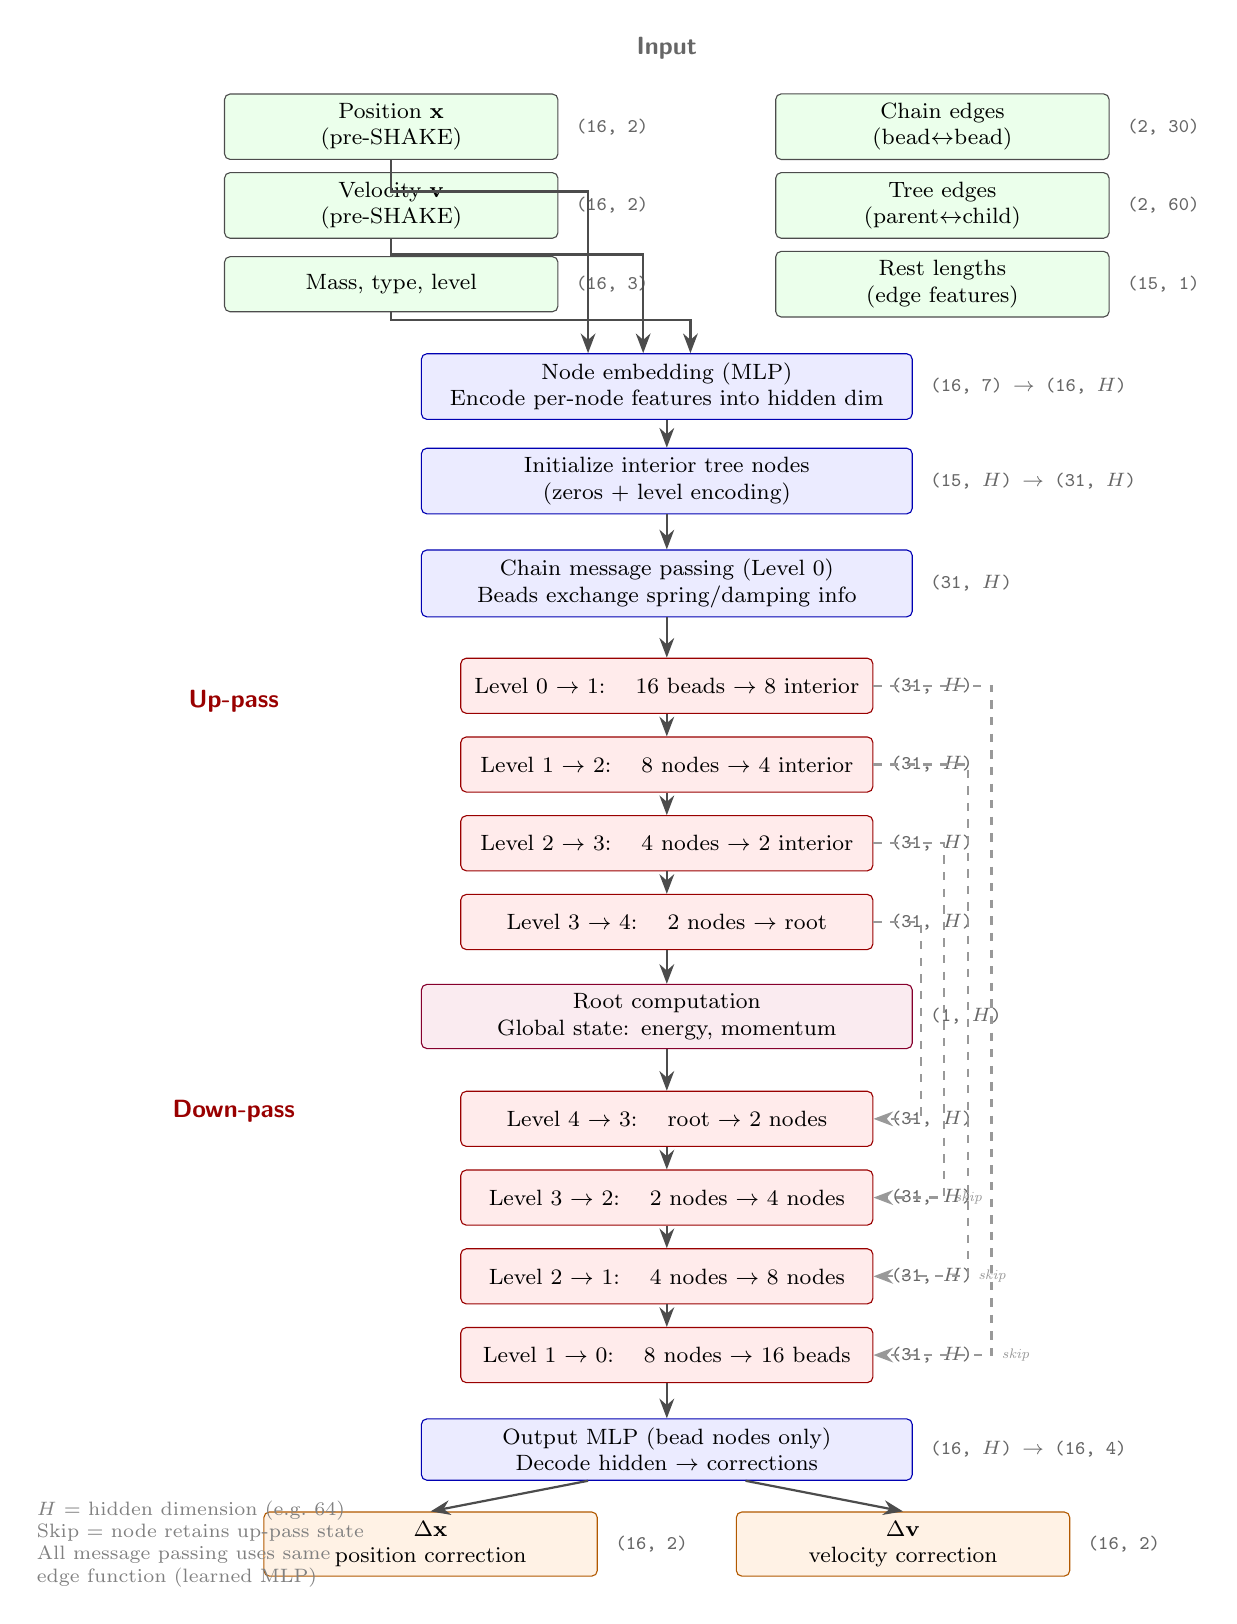
\begin{tikzpicture}[
    >={Stealth[length=2.5mm]},
    % Input/output boxes
    io/.style={
        rectangle, rounded corners=2pt, draw=black!70, fill=green!8,
        text width=4cm, minimum height=0.7cm, align=center,
        font=\footnotesize
    },
    % Processing boxes
    proc/.style={
        rectangle, rounded corners=2pt, draw=blue!70!black, fill=blue!8,
        text width=4.5cm, minimum height=0.7cm, align=center,
        font=\footnotesize
    },
    % Tree level boxes
    level/.style={
        rectangle, rounded corners=2pt, draw=red!60!black, fill=red!8,
        minimum height=0.7cm, align=center,
        font=\footnotesize
    },
    % Tensor label
    tensor/.style={
        font=\scriptsize\ttfamily, text=black!60
    },
    % Arrow
    arr/.style={->, thick, black!70},
    % Dashed arrow
    darr/.style={->, thick, black!40, dashed},
]

% ===== INPUT SECTION =====
\node[font=\small\bfseries\sffamily, text=black!60] at (0, 0.5) {Input};

\node[io] (in_pos) at (-3.5, -0.5)
    {Position $\mathbf{x}$ \\ (pre-SHAKE)};
\node[tensor, right=0.1cm of in_pos] {(16, 2)};

\node[io] (in_vel) at (-3.5, -1.5)
    {Velocity $\mathbf{v}$ \\ (pre-SHAKE)};
\node[tensor, right=0.1cm of in_vel] {(16, 2)};

\node[io] (in_scalar) at (-3.5, -2.5)
    {Mass, type, level};
\node[tensor, right=0.1cm of in_scalar] {(16, 3)};

\node[io] (in_edge) at (3.5, -0.5)
    {Chain edges \\ (bead$\leftrightarrow$bead)};
\node[tensor, right=0.1cm of in_edge] {(2, 30)};

\node[io] (in_tree) at (3.5, -1.5)
    {Tree edges \\ (parent$\leftrightarrow$child)};
\node[tensor, right=0.1cm of in_tree] {(2, 60)};

\node[io] (in_rest) at (3.5, -2.5)
    {Rest lengths \\ (edge features)};
\node[tensor, right=0.1cm of in_rest] {(15, 1)};

% ===== NODE EMBEDDING =====
\node[proc, text width=6cm] (embed) at (0, -3.8)
    {Node embedding (MLP) \\ Encode per-node features into hidden dim};
\node[tensor, right=0.1cm of embed] {(16, 7) $\to$ (16, $H$)};

\draw[arr] (in_pos.south) -- ++(0,-0.4) -| ([xshift=-1cm]embed.north);
\draw[arr] (in_vel.south) -- ++(0,-0.2) -| ([xshift=-0.3cm]embed.north);
\draw[arr] (in_scalar.south) -- ++(0,-0.1) -| ([xshift=0.3cm]embed.north);

% ===== INITIALIZE TREE NODES =====
\node[proc, text width=6cm] (init_tree) at (0, -5.0)
    {Initialize interior tree nodes \\ (zeros + level encoding)};
\node[tensor, right=0.1cm of init_tree] {(15, $H$) $\to$ (31, $H$)};

\draw[arr] (embed) -- (init_tree);

% ===== CHAIN MESSAGE PASSING =====
\node[proc, text width=6cm] (chain_mp) at (0, -6.3)
    {Chain message passing (Level 0) \\ Beads exchange spring/damping info};
\node[tensor, right=0.1cm of chain_mp] {(31, $H$)};

\draw[arr] (init_tree) -- (chain_mp);

% ===== UP-PASS =====
\node[font=\small\bfseries\sffamily, text=red!60!black] at (-5.5, -7.8) {Up-pass};

\node[level, text width=5cm] (up1) at (0, -7.6)
    {Level 0 $\to$ 1: \; 16 beads $\to$ 8 interior};
\node[tensor, right=0.1cm of up1] {(31, $H$)};

\node[level, text width=5cm] (up2) at (0, -8.6)
    {Level 1 $\to$ 2: \; 8 nodes $\to$ 4 interior};
\node[tensor, right=0.1cm of up2] {(31, $H$)};

\node[level, text width=5cm] (up3) at (0, -9.6)
    {Level 2 $\to$ 3: \; 4 nodes $\to$ 2 interior};
\node[tensor, right=0.1cm of up3] {(31, $H$)};

\node[level, text width=5cm] (up4) at (0, -10.6)
    {Level 3 $\to$ 4: \; 2 nodes $\to$ root};
\node[tensor, right=0.1cm of up4] {(31, $H$)};

\draw[arr] (chain_mp) -- (up1);
\draw[arr] (up1) -- (up2);
\draw[arr] (up2) -- (up3);
\draw[arr] (up3) -- (up4);

% ===== ROOT =====
\node[proc, text width=6cm, draw=purple!70!black, fill=purple!8] (root) at (0, -11.8)
    {Root computation \\ Global state: energy, momentum};
\node[tensor, right=0.1cm of root] {(1, $H$)};

\draw[arr] (up4) -- (root);

% ===== DOWN-PASS =====
\node[font=\small\bfseries\sffamily, text=red!60!black] at (-5.5, -13.0) {Down-pass};

\node[level, text width=5cm] (dn4) at (0, -13.1)
    {Level 4 $\to$ 3: \; root $\to$ 2 nodes};
\node[tensor, right=0.1cm of dn4] {(31, $H$)};

\node[level, text width=5cm] (dn3) at (0, -14.1)
    {Level 3 $\to$ 2: \; 2 nodes $\to$ 4 nodes};
\node[tensor, right=0.1cm of dn3] {(31, $H$)};

\node[level, text width=5cm] (dn2) at (0, -15.1)
    {Level 2 $\to$ 1: \; 4 nodes $\to$ 8 nodes};
\node[tensor, right=0.1cm of dn2] {(31, $H$)};

\node[level, text width=5cm] (dn1) at (0, -16.1)
    {Level 1 $\to$ 0: \; 8 nodes $\to$ 16 beads};
\node[tensor, right=0.1cm of dn1] {(31, $H$)};

\draw[arr] (root) -- (dn4);
\draw[arr] (dn4) -- (dn3);
\draw[arr] (dn3) -- (dn2);
\draw[arr] (dn2) -- (dn1);

% Skip connections
\draw[darr] (up1.east) -- ++(1.5, 0) |- (dn1.east)
    node[midway, right, font=\tiny\itshape, text=black!40] {skip};
\draw[darr] (up2.east) -- ++(1.2, 0) |- (dn2.east)
    node[midway, right, font=\tiny\itshape, text=black!40] {skip};
\draw[darr] (up3.east) -- ++(0.9, 0) |- (dn3.east)
    node[midway, right, font=\tiny\itshape, text=black!40] {skip};
\draw[darr] (up4.east) -- ++(0.6, 0) |- (dn4.east);

% ===== OUTPUT SECTION =====
\node[proc, text width=6cm] (decode) at (0, -17.3)
    {Output MLP (bead nodes only) \\ Decode hidden $\to$ corrections};
\node[tensor, right=0.1cm of decode] {(16, $H$) $\to$ (16, 4)};

\draw[arr] (dn1) -- (decode);

\node[io, fill=orange!10, draw=orange!70!black] (out_pos) at (-3, -18.5)
    {$\Delta\mathbf{x}$ \\ position correction};
\node[tensor, right=0.1cm of out_pos] {(16, 2)};

\node[io, fill=orange!10, draw=orange!70!black] (out_vel) at (3, -18.5)
    {$\Delta\mathbf{v}$ \\ velocity correction};
\node[tensor, right=0.1cm of out_vel] {(16, 2)};

\draw[arr] ([xshift=-1cm]decode.south) -- (out_pos.north);
\draw[arr] ([xshift=1cm]decode.south) -- (out_vel.north);

% ===== NOTES =====
\node[font=\scriptsize, text=black!50, text width=5cm, align=left]
    at (-5.5, -18.5) {
    $H$ = hidden dimension (e.g.\ 64)\\
    Skip = node retains up-pass state\\
    All message passing uses same\\
    edge function (learned MLP)
};

\end{tikzpicture}
\caption{U-Net GNN architecture with tensor shapes. Green boxes: input data.
Blue boxes: processing steps. Red boxes: tree message-passing levels.
Purple box: root computation (global). Orange boxes: output predictions.
Dashed arrows indicate skip connections (each node retains its up-pass state
for use during the down-pass). Hidden dimension $H$ is a hyperparameter.
The model takes the unconstrained state after integration and predicts the
SHAKE corrections $(\Delta\mathbf{x}, \Delta\mathbf{v})$ for each bead.}
\label{fig:unet_model}
\end{figure}

% ==========================================================================
\section{Changelog}
\label{sec:changelog}
% ==========================================================================

\begin{description}
    \item[2026-03-14] Added Qt/C++ architecture section documenting per-bead
          (node-local) vs.\ global operations with GNN analogues. Added
          binary-tree GNN plan for hierarchical message passing. Updated
          simulation to 16 beads, tapered mass, SHAKE constraints, and
          global drag.
    \item[2026-03-12] Initial report. Documented SHAKE (failed) and
          symplectic Euler (successful) formulations. Simulation validated
          for energy conservation and constraint fidelity. GNN-ready data
          export implemented.
\end{description}

\end{document}
